\label{sec:2.1}

%%%%%%%%%%%%%%%%
% (LIN) CTS
%%%%%%%%%%%%%%%%

The Cryogenic Test System (CTS) was built by a group from the Michigan State University. The CTS allows user to thermal cycle the ASIC from room to cryogenic temperature. Each lab has at least one CTS unit for testing the ColdADC in LN$_2$. Figure~\ref{fig:cts} shows the CTS.
\begin{figure}[htb]
\centering
%\begin{minipage}[b]{1.0\textwidth}
\begin{center}
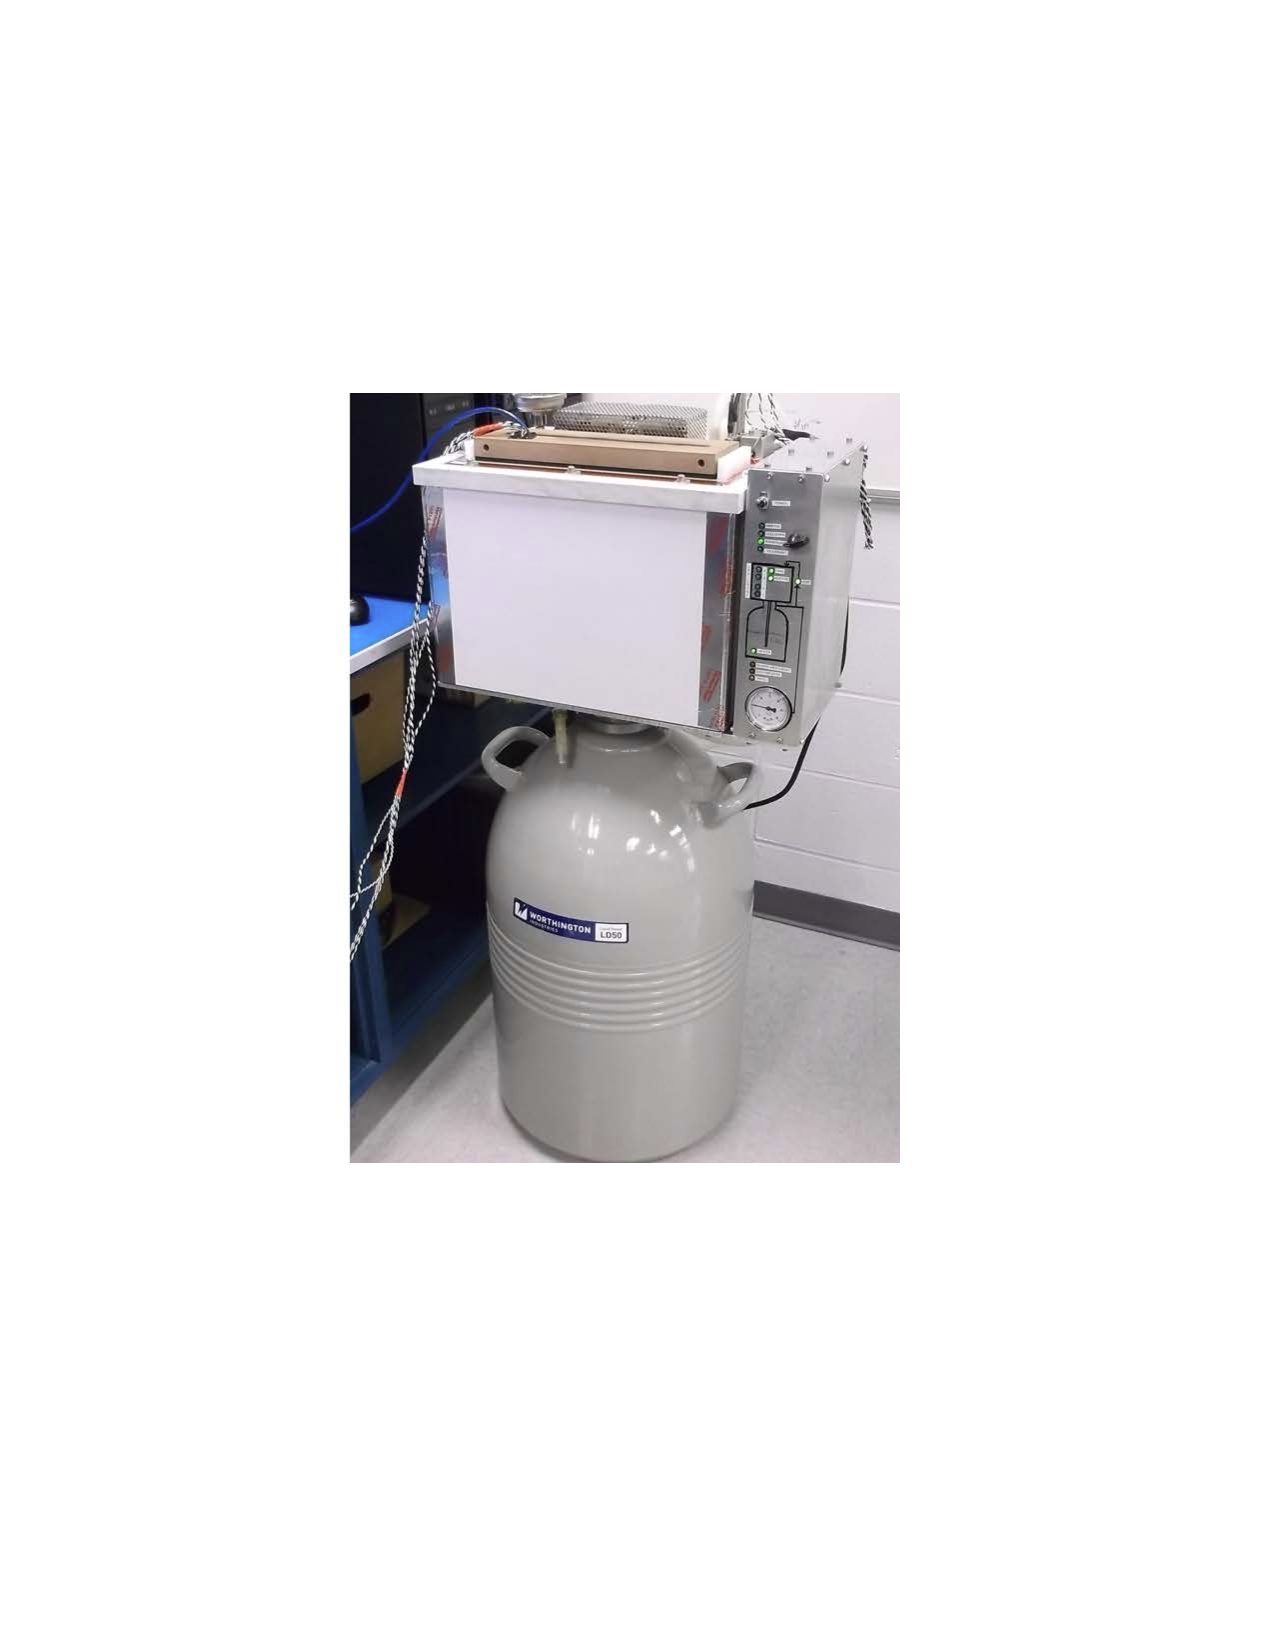
\includegraphics[width=0.5\textwidth]{figures/CTS.pdf}
\end{center}
%\end{minipage}
\caption{Cryogenic Test System.}
\label{fig:cts}
\end{figure}

